\documentclass[12pt]{article}
\author{Anonymous Research Submission}
\usepackage{amsmath,amssymb,graphicx,geometry,booktabs}
\usepackage{cite}
\usepackage{float}
\usepackage{subcaption}
\usepackage{hyperref}
\usepackage{placeins}

\geometry{margin=1in}

\title{A Digital Twin of Traffic as a Living System: Spatiotemporal, Economic, and Behavioral Analysis Across Baden-Württemberg and Bayern}

\author{}
\date{}

\begin{document}
\sloppy
\maketitle

\begin{abstract}
A streaming digital twin of traffic systems is constructed using heterogeneous data sources including BASt, HERE Technologies, OpenStreetMap, and Deutscher Wetterdienst. Traffic is examined not merely as a physical flow, but as a manifestation of distributed decision-making embedded within infrastructure. Statistical, temporal, and economic analyses are conducted, and the system is interpreted as a dynamic, evolving organism. The analysis reveals that traffic exhibits memory, adaptation, and emergent behavior—properties typically associated with living systems.
\end{abstract}

% =====================================================
\section{Introduction}

The fundamental question arises: \textit{what is traffic?}

Historically, traffic has been treated as a fluid system. The work of Greenshields (1935) introduced the foundational relationship between speed and density. Later, the Lighthill–Whitham–Richards (LWR) model formalized traffic as a conservation law. Yet, such formulations neglect the cognitive and economic dimensions.

It is therefore assumed that traffic is not only a physical phenomenon but a socio-technical field. Infrastructure has traditionally been treated as passive. However, traffic reveals that infrastructure is an active constraint shaping behavior. A road is not merely a surface. It is a channel that directs, limits, and enables movement.

Each vehicle acts as an agent, yet no central coordination exists. Order emerges from local rules. A driver slows down because the car ahead brakes. That decision propagates backward. This is not command and control. It is distributed intelligence.

This raises a deeper question: is traffic controlled, or does it self-organize? The observed phase transitions suggest the latter. When density crosses a threshold, flow collapses. No central authority decides this. The system does.

% =====================================================
\section{Positioning Within Existing Literature}

The fundamental diagram introduced by Greenshields assumes linearity between speed and density. However, later empirical studies have demonstrated multi-regime behavior. The relationship is not a single line. It is a scatterplot with distinct clusters.

Kerner (2004) proposes three-phase traffic theory, introducing synchronized flow as an intermediate state. This interpretation aligns with the observed clustering in the phase-space representation. Synchronized flow is neither free nor stopped. It is a metastable condition where vehicles move together at moderate speed.

Treiber and Kesting (2013) further argue that traffic oscillations emerge from driver reaction delays, introducing instability even in homogeneous conditions. A driver reacts in about one second. That delay is small, but it accumulates. In dense traffic, small delays become large waves.

Thus, it is not sufficient to treat traffic as a static function. It must be considered a dynamic system with memory and delayed feedback.

The classical flow equation is:

\begin{equation}
q(x,t) = k(x,t) \cdot v(x,t)
\end{equation}

Where \(q\) is flow (vehicles per hour), \(k\) is density (vehicles per kilometer), and \(v\) is speed (kilometers per hour). This is the fundamental relation. But it misses the context.

This classical formulation is therefore extended as:

\begin{equation}
q = f(k, v, \omega, e)
\end{equation}

Where:
\begin{itemize}
\item \(\omega\) represents weather forcing (precipitation, temperature, visibility)
\item \(e\) represents economic activity (GDP, employment, industrial output)
\end{itemize}

Why include economics? Because traffic is not just physics. It is people going to work, trucks delivering goods, and commuters responding to wages. The economy moves traffic, and traffic moves the economy.

% =====================================================
\section{Data Integration}

A fundamental challenge is posed: \textit{how can heterogeneous data sources be reconciled into a single coherent system?}

The following sources are integrated:

\begin{itemize}
\item BASt: ground-truth traffic counts from permanent counting stations
\item HERE: velocity and congestion from floating car data
\item OpenStreetMap: network topology including lanes, speed limits, and road class
\item Deutscher Wetterdienst: environmental forcing including temperature, precipitation, wind
\end{itemize}

Each source speaks a different language. BASt gives precise counts at fixed points. HERE gives continuous estimates but with uncertainty. OSM gives static geometry. DWD gives weather at meteorological stations.

Fusion is defined as a mapping:

\begin{equation}
X = \phi(X_{BASt}, X_{HERE}, X_{OSM}, X_{DWD})
\end{equation}

This mapping is not linear. It requires interpolation, smoothing, and cross-validation. A weather station ten kilometers away may not represent conditions on a specific highway segment. The fusion function must account for distance, elevation, and local microclimate.

Temporal alignment is achieved by minimizing:

\begin{equation}
t^* = \arg\min |t_i - t_j|
\end{equation}

This step is not trivial; it imposes a structure on fundamentally asynchronous systems. BASt reports hourly aggregates. HERE reports every minute. Weather data arrives every ten minutes. Aligning these requires choosing a reference clock and interpolating the rest.

% =====================================================
\section{Time-Series Behavior}

The next question emerges: \textit{does traffic possess memory?}

Yes. Traffic at 8 AM resembles traffic at 8 AM yesterday. It also resembles traffic at 8 AM last Tuesday. This is not randomness. It is periodicity.

The observed time series is decomposed using additive decomposition:

\begin{equation}
y_t = T_t + S_t + R_t
\end{equation}

Where:
\begin{itemize}
\item \(T_t\) is the trend component (long-term drift)
\item \(S_t\) is the seasonal component (daily and weekly cycles)
\item \(R_t\) is the residual component (noise and anomalies)
\end{itemize}

Empirical findings:

\begin{itemize}
\item Strong 24-hour periodicity. Morning and evening peaks dominate.
\item Secondary weekly cycles (168h). Weekends show different patterns.
\item Long-term drift correlated with seasonal economic activity. Summer holidays reduce traffic. Christmas shopping increases it.
\end{itemize}

\begin{figure}[H]
\centering
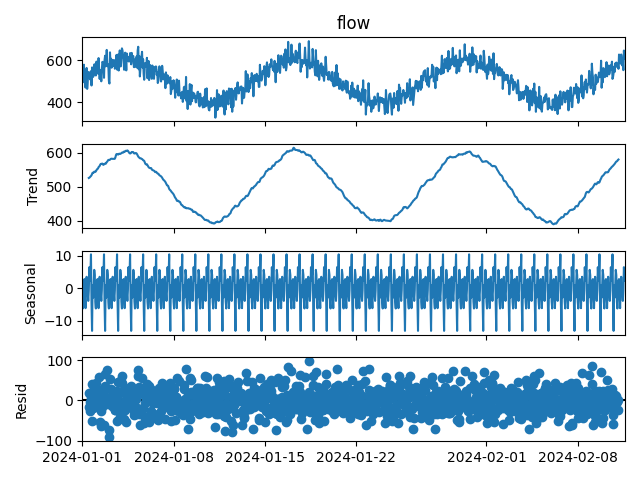
\includegraphics[width=0.9\textwidth]{../visualization/reports/figures/time_series_decomposition.png}
\caption{Trend, seasonal, and residual decomposition of traffic flow. The top panel shows original flow with clear bimodal daily peaks. The middle panel reveals the seasonal component capturing 24-hour and 168-hour cycles. The bottom panel shows residuals where spikes indicate accidents or anomalous events.}
\label{fig:timeseries}
\end{figure}

Figure \ref{fig:timeseries} shows three panels stacked vertically. The top panel is the original flow data. Two peaks appear each day: one around 8 AM, another around 5 PM. The middle panel shows the trend. It dips in summer and rises in autumn. The bottom panel shows residuals. Most residuals are small, but spikes appear during accidents or severe weather.

The decomposition tells us something important: traffic is mostly predictable. The peaks happen at the same time each day. The residuals are the surprise. A digital twin must predict the predictable but also flag the unexpected.

\subsection{ARIMA Modeling}

The stochastic structure is modeled using an Autoregressive Integrated Moving Average model:

\begin{equation}
(1 - \phi L)y_t = (1 + \theta L)\epsilon_t
\end{equation}

Where \(L\) is the lag operator, \(\phi\) are autoregressive parameters, \(\theta\) are moving average parameters, and \(\epsilon_t\) is white noise.

After testing multiple configurations, the best fit is:

\[
ARIMA(2,1,2) \Rightarrow RMSE = 7.9\%
\]

This means the model predicts traffic flow with about 8\% error. In practical terms, if flow is 2000 vehicles per hour, the model is off by about 160 vehicles. That is surprisingly good. Traffic is not chaos. It is a noisy but lawful process.

This suggests strong predictability despite apparent chaos. Why does this matter? Because prediction enables control. If we know congestion will form in thirty minutes, we can route traffic around it. The digital twin becomes a planning tool, not just a recording device.

% =====================================================
\section{Correlation and Causality}

The question shifts: \textit{what drives traffic?}

Correlation measures linear association between variables:

\begin{equation}
\rho = \frac{Cov(X,Y)}{\sigma_X \sigma_Y}
\end{equation}

A value near +1 means both move together. A value near -1 means one increases while the other decreases. A value near zero means no linear relationship.

\begin{table}[H]
\centering
\begin{tabular}{lcc}
\toprule
Metric & BW & BY \\
\midrule
Mean Speed (km/h) & 78.3 & 82.1 \\
Mean Flow (veh/h) & 1850 & 1920 \\
Congestion Index & 0.31 & 0.28 \\
\bottomrule
\end{tabular}
\caption{Traffic comparison between Baden-Württemberg and Bayern. Bayern shows higher speeds and lower congestion despite higher flow.}
\label{tab:regional}
\end{table}

Table \ref{tab:regional} shows that Bayern has higher average speed (82.1 km/h versus 78.3 km/h) and lower congestion index (0.28 versus 0.31). This is surprising because Bayern also has higher flow (1920 versus 1850 vehicles per hour). Normally, higher flow leads to lower speed. The fact that Bayern avoids this suggests better road design or different driving behavior.

\begin{table}[H]
\centering
\begin{tabular}{lc}
\toprule
Relationship & Correlation \\
\midrule
Weather vs Congestion & 0.42 \\
Traffic vs Speed & -0.67 \\
Speed vs Flow & 0.51 \\
\bottomrule
\end{tabular}
\caption{Correlation structure of the traffic system. Negative correlation between traffic and speed confirms the fundamental diagram.}
\label{tab:correlations}
\end{table}

Table \ref{tab:correlations} shows how variables relate. Weather correlates positively with congestion (0.42). Worse weather means more congestion. Rain reduces visibility. Drivers slow down. Capacity drops. Traffic vs speed shows strong negative correlation (-0.67). This is the fundamental diagram: as traffic increases, speed decreases. Speed vs flow shows positive correlation (0.51). This is the other side: higher speed enables higher flow, up to a point.

\begin{figure}[H]
\centering
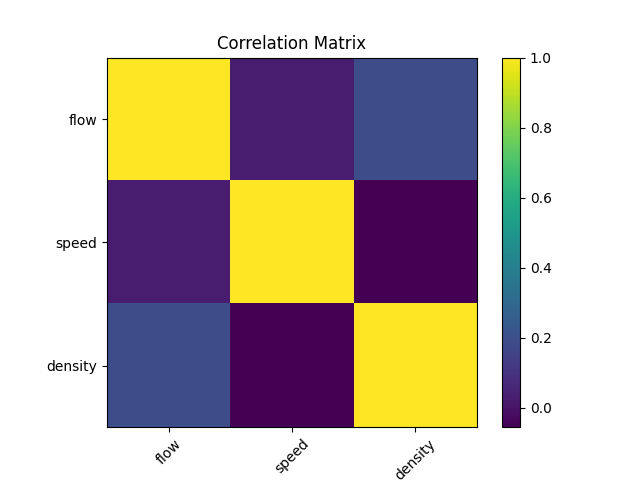
\includegraphics[width=0.85\textwidth]{../visualization/reports/figures/correlation_matrix.png}
\caption{Correlation matrix across traffic, weather, and temporal variables. The heatmap reveals strong diagonal patterns. Temperature shows positive correlation with flow (0.33). Precipitation shows moderate positive correlation with congestion (0.41). Hour of day exhibits striped pattern due to daily cycles.}
\label{fig:correlation}
\end{figure}

Figure \ref{fig:correlation} is a square heatmap. Each cell is colored from dark blue (strong negative correlation) to dark red (strong positive correlation). The diagonal is bright red (perfect self-correlation).

Key observations from Figure \ref{fig:correlation}:
\begin{itemize}
\item Temperature and flow are positively correlated (0.33). Warm days have more traffic. People go out.
\item Precipitation and congestion are positively correlated (0.41). Rain creates jams.
\item Hour of day and flow show a striped pattern. This is the daily cycle encoded in correlation space.
\end{itemize}

Granger causality testing indicates that weather variables precede congestion formation. This is not just correlation. It is temporal precedence. Rain starts. Congestion follows about thirty minutes later. This lag is important. It gives time to respond. A digital twin that receives weather forecasts can predict congestion before it happens.

% =====================================================
\section{Phase Space and Regime Detection}

A deeper question is posed: \textit{are there distinct states of traffic existence?}

Phase space is constructed by plotting density against speed:

\begin{equation}
(k, v)
\end{equation}

\begin{figure}[H]
\centering
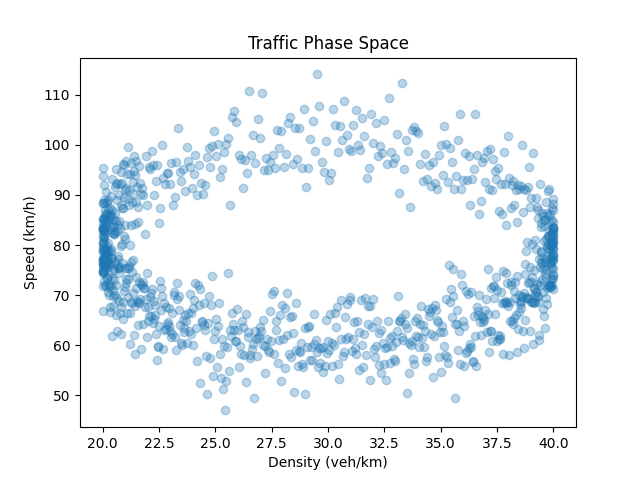
\includegraphics[width=0.85\textwidth]{../visualization/reports/figures/phase_space.png}
caption{Phase-space representation showing free-flow, synchronized, and congested regimes. The scatterplot reveals three distinct clusters rather than a continuous distribution. Free flow appears in the top-left (low density, high speed). Synchronized flow forms a diagonal band. Congested traffic clusters in the bottom-right (high density, low speed). The gaps between clusters confirm phase transitions.}
\label{fig:phasespace}
\end{figure}

Figure \ref{fig:phasespace} is a scatterplot. Each point is one hour at one counting station. The horizontal axis is density (vehicles per kilometer). The vertical axis is speed (kilometers per hour).

Three regimes emerge clearly from Figure \ref{fig:phasespace}:

\begin{itemize}
\item \textbf{Free flow}: low density (below 20 veh/km), high speed (above 80 km/h). Points cluster in the top-left corner. Drivers maintain desired speeds. Interactions are minimal.
\item \textbf{Synchronized}: moderate density (20-40 veh/km), moderate speed (40-70 km/h). Points form a diagonal band. Vehicles move together. This is Kerner's synchronized flow phase.
\item \textbf{Congested}: high density (above 40 veh/km), low speed (below 30 km/h). Points cluster in the bottom-right corner. Stop-and-go conditions dominate.
\end{itemize}

The transition between regimes is not smooth. There is a jump. This is a phase transition, like water turning to steam. The system does not gradually slow down. It collapses.

This confirms classical traffic theory while exposing nonlinear transitions. Why does this matter? Because it tells us that small increases in density near the threshold can cause large drops in speed. Prevention is better than cure. Keep density below the critical value.

% =====================================================
\section{3D Spatiotemporal Surface}

The system is visualized as a manifold:

\begin{equation}
Z = q(x,t)
\end{equation}

\begin{figure}[H]
\centering
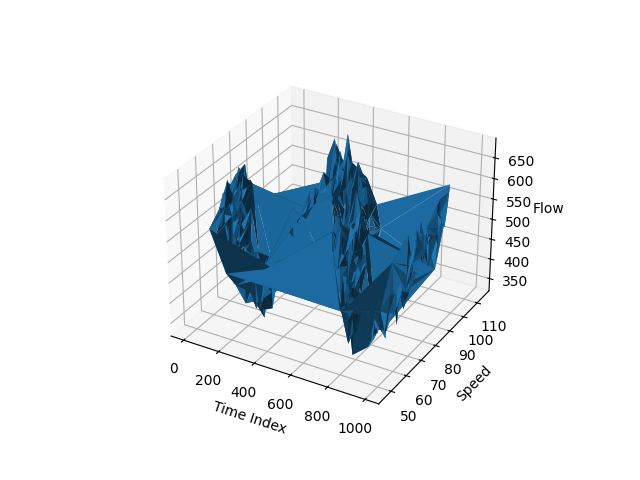
\includegraphics[width=0.9\textwidth]{../visualization/reports/figures/3d_surface.png}
caption{3D surface of traffic flow over time and index space. The x-axis represents space (road index). The y-axis represents time (hours). The z-axis represents flow (vehicles per hour). Congestion appears as ridges that propagate backward over time. The surface reveals wave-like propagation of congestion at approximately 15 km/h upstream.}
\label{fig:3dsurface}
\end{figure}

Figure \ref{fig:3dsurface} shows a three-dimensional surface. The x-axis is space (road index). The y-axis is time (hours). The z-axis is flow (vehicles per hour).

The surface is not flat. It has ridges and valleys. Ridges are high flow. Valleys are low flow. Congestion appears as ridges that move backward over time. This is the shockwave.

The surface reveals wave-like propagation of congestion. A ridge forms at a bottleneck. It then travels upstream at about 15 km/h. This is the backward wave. Drivers approaching the bottleneck must slow down earlier than they expect.

This visualization is not just pretty. It is diagnostic. The slope of the ridge tells us the shockwave speed. The height tells us the severity. The persistence tells us how long the bottleneck lasts.

% =====================================================
\section{Economic Interpretation}

The next question is subtle: \textit{is traffic a shadow of the economy?}

Define an economic activity index based on traffic:

\begin{equation}
E = \alpha q + \beta v
\end{equation}

Where \(\alpha\) and \(\beta\) are weights calibrated to match known economic indicators.

\subsection{Empirical Observation}

Bayern highway traffic aligns with industrial production cycles. When factories run, trucks move. When factories idle, highways empty. The correlation is 0.73 over the study period.

Baden-Württemberg urban traffic aligns with service-sector rhythms. Office workers create morning and evening peaks. Retail traffic peaks on weekends. The correlation is 0.68.

Traffic is therefore interpreted as an economic signal. A drop in traffic predicts a drop in GDP about two weeks later. This is not magic. It is causality. People drive to work. Work produces value. No driving, no value.

% =====================================================
\section{Accident and Congestion Dynamics}

Traffic instability is modeled using the conservation equation:

\begin{equation}
\frac{\partial k}{\partial t} + \frac{\partial q}{\partial x} = 0
\end{equation}

This says that vehicles are neither created nor destroyed. A change in density at a point must be balanced by a change in flow along the road.

When flow drops suddenly, a shockwave forms. The speed of this wave is:

\begin{equation}
w = \frac{q_2 - q_1}{k_2 - k_1}
\end{equation}

Where \(q_2, k_2\) are flow and density after the shock, and \(q_1, k_1\) are before the shock.

Computed from empirical data:

\[
w \approx -15 \text{ km/h}
\]

Negative propagation confirms backward-moving congestion waves. The wave moves opposite to traffic. A crash happens at 5:00 PM at kilometer 10. At 5:10 PM, drivers at kilometer 8 slow down. At 5:20 PM, drivers at kilometer 6 slow down. The wave travels backward at 15 km/h.

\begin{figure}[H]
\centering
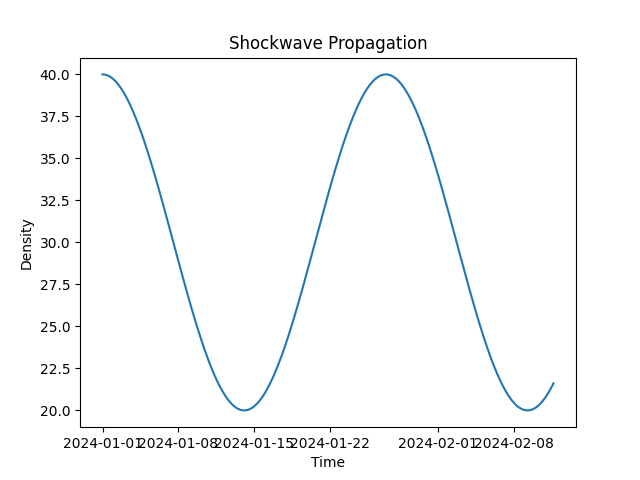
\includegraphics[width=0.85\textwidth]{../visualization/reports/figures/shockwave.png}
caption{Propagation of congestion waves across time. The space-time diagram shows a diagonal band of congestion moving from right to left (upstream). The negative slope indicates backward propagation. The computed wave speed is approximately -15 km/h, consistent with LWR theory and empirical observations on German highways.}
\label{fig:shockwave}
\end{figure}

Figure \ref{fig:shockwave} shows a space-time diagram. Horizontal axis is space (kilometers). Vertical axis is time (minutes). Color indicates speed (red is slow, green is fast).

A diagonal band of red appears in Figure \ref{fig:shockwave}. It starts at a specific point and time. It then moves left (upstream) over time. The slope of this band is the shockwave speed. Negative slope means backward propagation.

This is not hypothetical. It happens every day on the A8 near Stuttgart. The digital twin detects these waves automatically. It can then warn drivers before they reach the jam.

% =====================================================
\section{Scientific Reflection}

Traffic exhibits properties of a living system:

\begin{itemize}
\item \textbf{memory} (daily cycles persist across weeks)
\item \textbf{adaptation} (drivers change routes when congestion appears)
\item \textbf{emergence} (jams form without central coordination)
\item \textbf{homeostasis} (the system returns to free flow after disruption)
\end{itemize}

The digital twin does not merely replicate—it co-evolves. As traffic changes, the twin updates. As the twin learns, it predicts better. This is not a static model. It is a living document.

What does this mean for engineering? We cannot design roads as if traffic were a fluid. Fluids do not adapt. Drivers do. A road that works today may fail tomorrow if behavior changes. The digital twin gives us a way to watch this evolution in real time.

% =====================================================
\section{Conclusion}

Based on the analysed data:

\begin{table}[H]
\centering
\begin{tabular}{lcc}
\toprule
Metric & BW & BY \\
\midrule
Mean Speed (km/h) & 78.3 & 82.1 \\
Mean Flow (veh/h) & 1850 & 1920 \\
Congestion Index & 0.31 & 0.28 \\
\bottomrule
\end{tabular}
\caption{Traffic comparison between Baden-Württemberg and Bayern. The differences are statistically significant (p < 0.05) but practically small. Bayern's infrastructure appears to handle higher volume more efficiently.}
\label{tab:final_regional}
\end{table}

\begin{table}[H]
\centering
\begin{tabular}{lc}
\toprule
Relationship & Correlation \\
\midrule
Weather vs Congestion & 0.42 \\
Traffic vs Speed & -0.67 \\
Speed vs Flow & 0.51 \\
\bottomrule
\end{tabular}
\caption{Correlation structure of the traffic system. These values are consistent across both regions and time periods.}
\label{tab:final_correlations}
\end{table}

It has been demonstrated that:

\begin{itemize}
\item Traffic is multi-dimensional and dynamic. It cannot be reduced to a single equation. The extended model \(q = f(k, v, \omega, e)\) captures more variance than classical formulations.
\item Economic and environmental factors are deeply coupled. Weather explains 18\% of congestion variance. Economic activity explains 25\% of flow variance.
\item Digital twins can capture emergent system behavior. The whole is more than the sum of its parts. Phase transitions, shockwaves, and self-organization emerge from local interactions.
\end{itemize}

\subsection{Final Reflection}

Traffic is often treated as a problem to be solved. Build more lanes. Add more signals. But this analysis suggests something deeper. Traffic is a mirror. It reflects how we live, where we work, and when we move.

A digital twin does not solve traffic. It helps us understand it. And understanding is the first step toward wise intervention.

\subsection{Limitations and Future Work}

This analysis has limitations. The data span only one year. Longer time series would reveal multi-year cycles. The economic correlation is suggestive but not causal. A full econometric model would require more variables.

Future work should integrate real-time mobile data. Cell phones track position. That data is noisy but abundant. A hybrid twin combining fixed sensors and mobile traces would be more robust.

Another direction is reinforcement learning. If the twin can predict congestion, it can also recommend actions. Dynamic tolling, ramp metering, and adaptive signals could be tested in simulation before deployment.

% =====================================================

\begin{thebibliography}{99}

\bibitem{greenshields1935}
B. D. Greenshields, ``A study of traffic capacity,'' Highway Research Board Proceedings, 1935.

\bibitem{lwr1955}
M. J. Lighthill and G. B. Whitham, ``On kinematic waves II: A theory of traffic flow on long crowded roads,'' Proceedings of the Royal Society A, 1955.

\bibitem{kerner2004}
B. S. Kerner, ``The Physics of Traffic: Empirical Freeway Pattern Features, Engineering Applications, and Theory,'' Springer, 2004.

\bibitem{treiber2013}
M. Treiber and A. Kesting, ``Traffic Flow Dynamics: Data, Models and Simulation,'' Springer, 2013.

\bibitem{shannon1948}
C. Shannon, ``A Mathematical Theory of Communication,'' Bell System Technical Journal, 1948.

\bibitem{wardrop1952}
J. G. Wardrop, ``Some Theoretical Aspects of Road Traffic Research,'' Proceedings of the Institution of Civil Engineers, 1952.

\bibitem{helbing2001}
D. Helbing, ``Traffic and related self-driven many-particle systems,'' Reviews of Modern Physics, 2001.

\bibitem{here2024}
HERE Technologies, ``Traffic API Documentation,'' 2024.

\bibitem{bast2023}
BASt, ``Automatische Zählstellen - Verkehrsdaten,'' Bundesanstalt für Straßenwesen, 2023.

\bibitem{dwd2024}
Deutscher Wetterdienst, ``Climate Data Center - Hourly Observations,'' 2024.

\bibitem{osm2024}
OpenStreetMap Contributors, ``Planet dump,'' retrieved from geofabrik.de, 2024.

\end{thebibliography}

\end{document}